\documentclass{article}
\usepackage{graphicx}
\usepackage{epsfig}
\usepackage{amssymb,amsmath}
\usepackage{array}
\graphicspath{ {Desktop} }
\setlength{\parindent}{0pt}
\title{CTA200 2020 Project Summary}
\author{SURP Student Ethan Sun}
\date{May 19th, 2020}

\begin{document}

\maketitle
\section*{1. Introuction}
The purpose of this project is to rederive the self similar solutions for a shock wave propagating through a medium with varying densities and reproduce the results found by Akira Sakurai. The problem can be separated into two parts. The first part considers the stage before the shock wave arrives at the boundary, while the second one deals with the subsequent expansion as the gas expands into vacuum. I will describe the steps I took while deriving the solutions and present the results from numerical integrations in the following sections.

\section*{2. Derivation}
The problem can be simplified into an one-dimensional case since we are studying the phenomena close to the gas boundary. 
\\
\centerline{\includegraphics[scale=0.6]{fig1.png}}
\\
\centerline{Figure 1}
\\
\bigbreak
\newpage
Figure 1 illustrates the proble in its first stage. The \textit{x}-axis points into the gas and is perpendicular to the boundary, \textit{x} = 0, where the initial density $\rho_0(\textit{x})$ = 0. The location of the shock wave is \textit{x} = $\textit{X}(\textit{t})$ and the shock wave travels in the negative \textit{x} direction with velocity \textit{U}: 
\begin{equation}
U = \frac{dX}{dt}
\end{equation}
The velocity \textit{u}, pressure \textit{p}, and desity $\rho$ satisfy the following equations derived from one-dimensional continuity equation, Newton's First Law, and polytropic relation:
\begin{equation}
\frac{D\rho}{Dt} = -\rho\frac{\partial u}{\partial x}
\end{equation}
\begin{equation}
\frac{Du}{Dt} = -\frac{1}{\rho}\frac{\partial p}{\partial x}+F_0
\end{equation}
\begin{equation}
\frac{Dp\rho^{-\gamma}}{Dt} = 0
\end{equation}
where $F_0$ is body force per unit mass and $\gamma$ is the polytropic index. By applying the chain rule and substituting equation (2) into equation (4), equation (4) can be simplified into:
\begin{equation}
\frac{Dp}{Dt} = -\gamma p\frac{\partial u}{\partial x}
\end{equation}
Since our area of interest is close to the gas boundary, it is reasonable to assume the density decreases as a power of \textit {x}:
\begin{equation}
\rho_0(x) = k_1x^\alpha
\end{equation}
When $F_0$ is zero, the solutions to equations (2), (3), (5) together with equation (6) can be found as a similarity solution under the category of progressing wave described by Courant and Friedrichs:
\begin{equation}
    \begin{split}
        u &= U(x)f(\eta) \\
        p &= \rho_0(x)U^2(x)g(\eta) \\
        \rho &= \rho_0(x)h(\eta)
    \end{split}
\end{equation}
with
\begin{equation}
\eta = (\frac{X}{x})^{\lambda+1}, (0\leqslant \eta \leqslant 1)
\end{equation}
and
\begin{equation}
U(X) = k_2X^{-\lambda}
\end{equation}
\newpage
where we assumed this tyoe of similarity solution in order to fit the singularity at $X = 0$. We can then obtain the following ODEs for \textit{f}, \textit{g}, \textit{h} by substituting equations (7), (8), (9) into equations (2), (3), (5):
\begin{equation}
    \begin{split}
        (1-\eta f)f^{'}-\eta \frac{g^{'}}{h} &= \frac{\lambda}{1+\lambda}f^{2}-\frac{\alpha-2\lambda}{1+\lambda}\frac{g}{h}\\
        (1-\eta f)\frac{h^{'}}{h}-\eta f^{'} &= -\frac{\alpha-\lambda}{1+\lambda}f\\
        (1-\eta f)\frac{g^{'}}{g}-\lambda\eta f^{'} &= -\frac{\alpha-(\gamma+2)\lambda}{1+\lambda}f
    \end{split}
\end{equation}
$\lambda$ could be proved to be positive and therefore \textit{U} becomes large as \textit{X} becomes small. Since density decreases, the speed of sound $\textit c_0$ is also small around $\textit x=0$. This means the Mach number is large at this location and a strog shock wave shall present. According to the Rankine-Huginot conditions, the following equations could be written at $\textit x=X$:
\begin{equation}
    \begin{split}
        (u)_{x=X} &= \frac{2}{\gamma+1}U(X) \\
        (p)_{x=X} &= \frac{2}{\gamma+1}\rho_{0}(X)U^{2}(X) \\
        (\rho)_{x=X} &= \rho_{0}(X)\frac{\gamma+1}{\gamma-1}
    \end{split}
\end{equation}
We could then obtain the following boundary conditions for \textit{f}, \textit{g}, \textit{h} at $\eta=1$ by comparing equation (7) with (11):
\begin{equation}
    \begin{split}
        f(1) &= \frac{2}{\gamma+1} \\
        g(1) &= \frac{2}{\gamma+1} \\
        h(1) &= \frac{\gamma+1}{\gamma-1}
    \end{split}
\end{equation}
However, a solution cannot be found as it always breaks down at a certain point $\eta_0$, except for one special $\lambda$ value. A set of approximated values of $\lambda$ for certain $\alpha$ and $\gamma$ values were determined using Whiham's method:
\\
\centerline{\includegraphics[scale=0.75]{fig2.png}}
\\
\centerline{Table 1}
\\
\bigbreak
\newpage
We could then numerically integrate equation (10) from $\eta=1$ to $\eta=0$ as shown in Section 3. The results obtained from Sakurai's work are as follows:
\\
\centerline{\includegraphics[scale=0.9]{fig3.png}}
\\
\centerline{Table 2}
\\
\bigbreak
Finally, we could obtain the distributions of velocity, pressure, and density $\textit{u}_1$, $\textit{p}_1$, $\rho_1$ behind the shock wave when $\textit{t}=0$ by setting $\eta=0$ in equation (7) and substituting the $\textit{f}(0)$, $\textit{g}(0)$, $\textit{h}(0)$ terms with the values we just found:
\begin{equation}
    \begin{split}
        u_{1} &= U(x)f(0) = f(0)k_{2}x^{-\lambda} \\
        p_{1} &= \rho_{0}(x)U^{2}(x)g(0) = g(0)k_{1}k_{2}^{2}x^{\alpha-2\lambda} \\
        \rho_{1} &= \rho_{0}(x)h(0) = h(0)k_{1}x^{\alpha}
    \end{split}
\end{equation}
The next step would be applying the similarity solution method again to the region where $\textit{x}\leqslant0$, as gas expands into the vacuum. We could also use the results we found in equation (13) as a initial condition for the new ODEs. However, I was not able to go through the derivation for this part due to the limited time. 

\section*{3. Numerical Integration}
The objective is to reproduce the integrations Sakurai performed in his work. I first simplified the ODEs in equation (10) into expressions of $\textit{f}^{'}$, $\textit{g}^{'}$ and $\textit{h}^{'}$. Ideally, the $scipy.integrate.solve\_bvp$ function should be able to solve this problem since we have all the boundary conditions at $\eta=1$. 
\bigbreak
However, among the multiple sets of initial guess I experimented, none of them could yield a valid solution curve similar to the ones presented in Sakurai's work. It is very likely that I wasn't applying this solving function correctly. I then decided to integrate the ODEs as an initial value problem instead. At this point what I was trying to do was simply reproducing the integrated results, rather than finding the $\textit{f}(0)$, $\textit{g}(0)$ and $\textit{h}(0)$ values as indicated before. Therefore, I relied on the values from Table 2 as my initial conditions and applied the solving function $scipy.integrate.odeint$. The resulting plots are as follows.
\newpage
\centerline{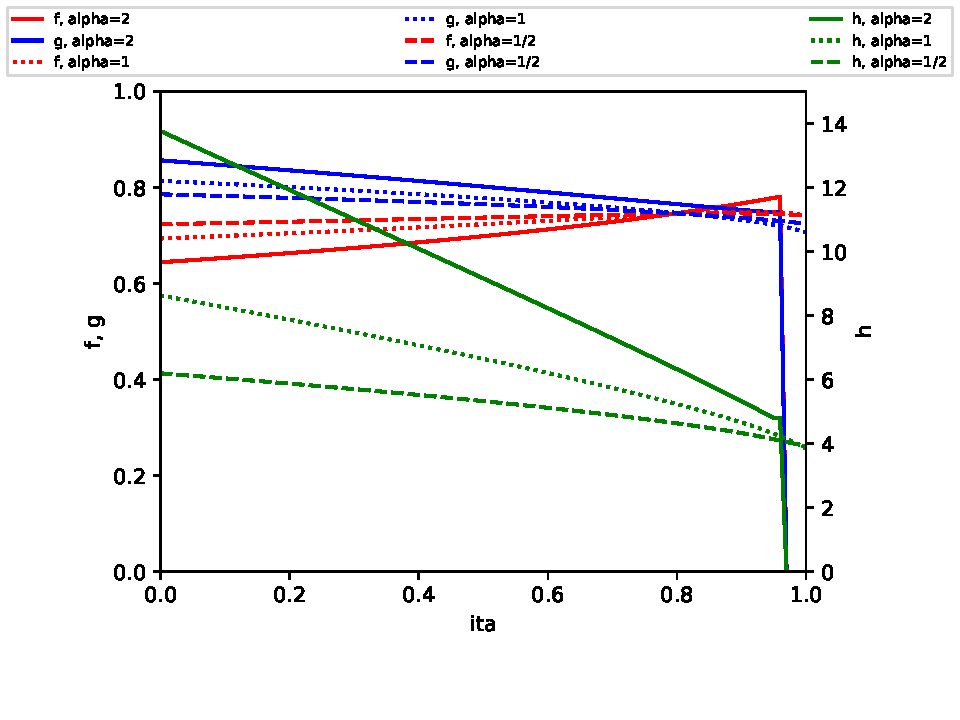
\includegraphics[scale=0.8]{gamma 1.67.pdf}}
\centerline{Figure 2.1: $\gamma$=$\frac{5}{3}$, reproduced}
\centerline{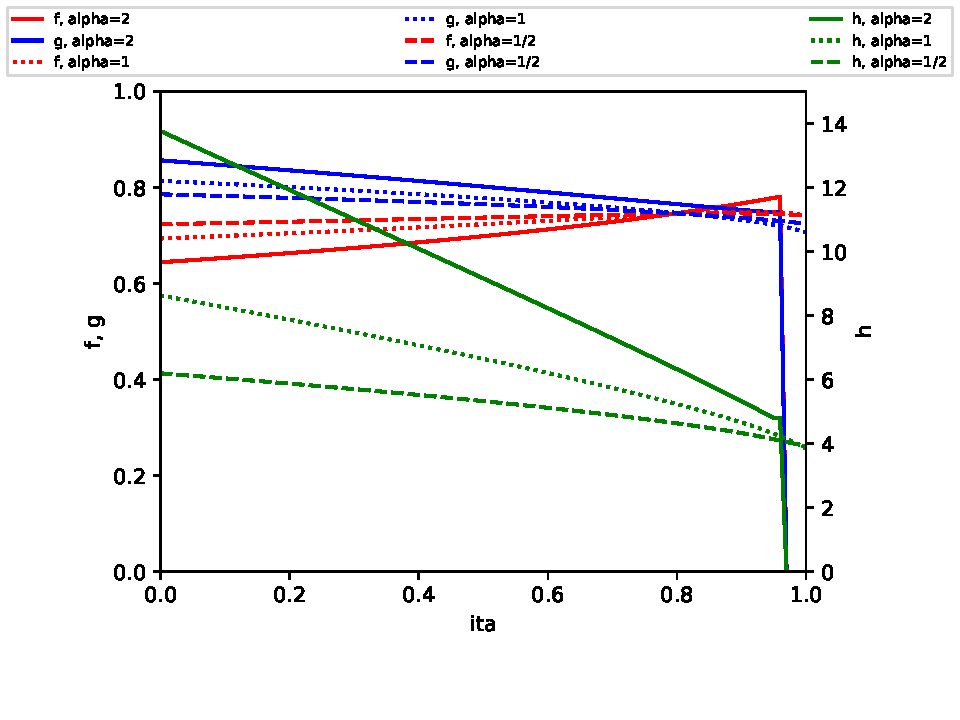
\includegraphics[scale=0.9]{gamma 1.67.png}}
\centerline{Figure 2.2: $\gamma$=$\frac{5}{3}$, Sakurai}

\newpage
\centerline{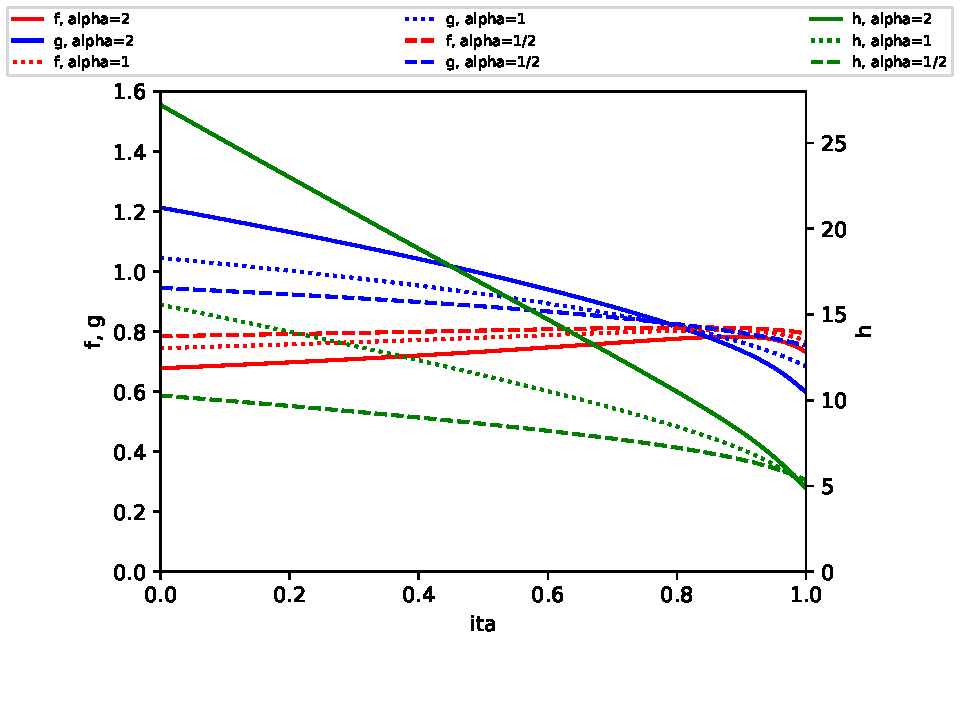
\includegraphics[scale=0.7]{gamma 1.4.pdf}}
\centerline{Figure 3.1: $\gamma$=$\frac{7}{5}$, reproduced}
\centerline{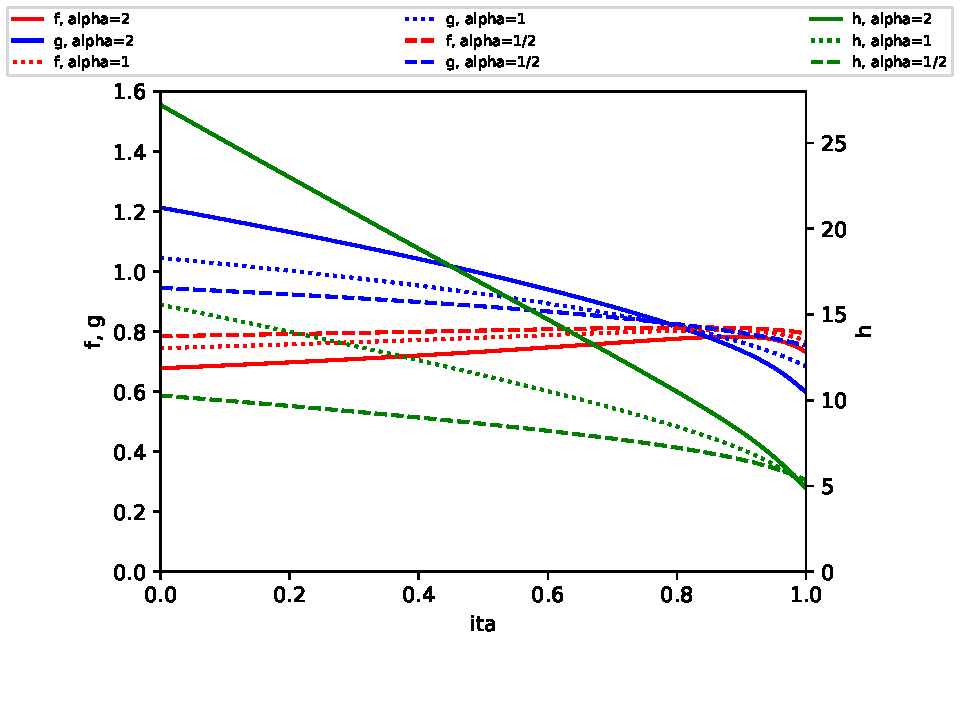
\includegraphics[scale=0.8]{gamma 1.4.png}}
\centerline{Figure 3.2: $\gamma$=$\frac{7}{5}$, Sakurai}

\newpage
\centerline{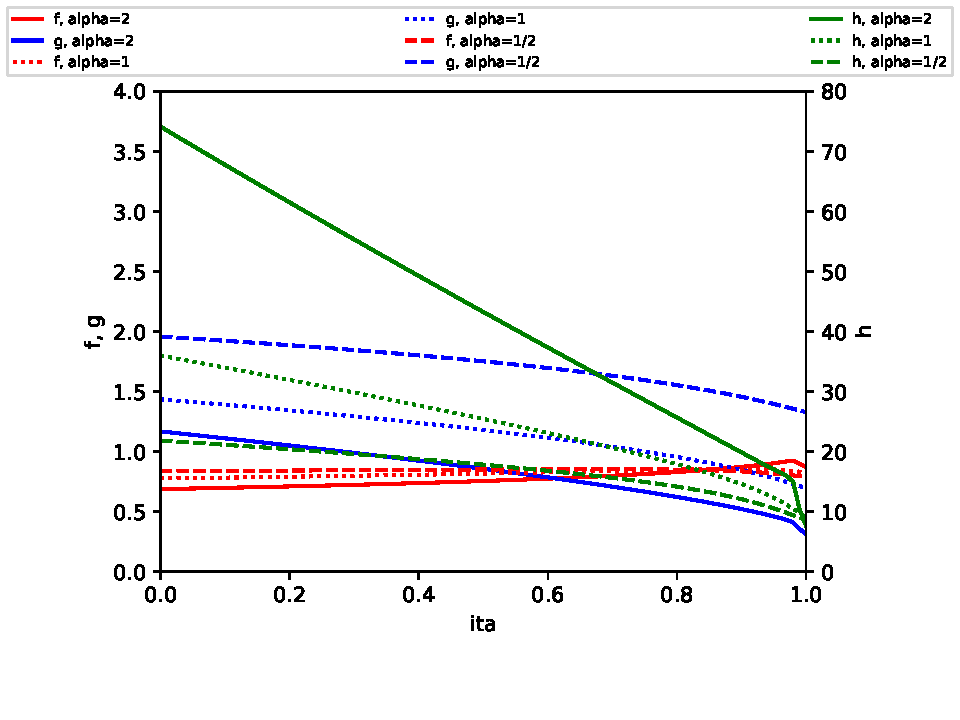
\includegraphics[scale=0.7]{gamma 1.2.pdf}}
\centerline{Figure 4.1: $\gamma$=$\frac{6}{5}$, reproduced}
\centerline{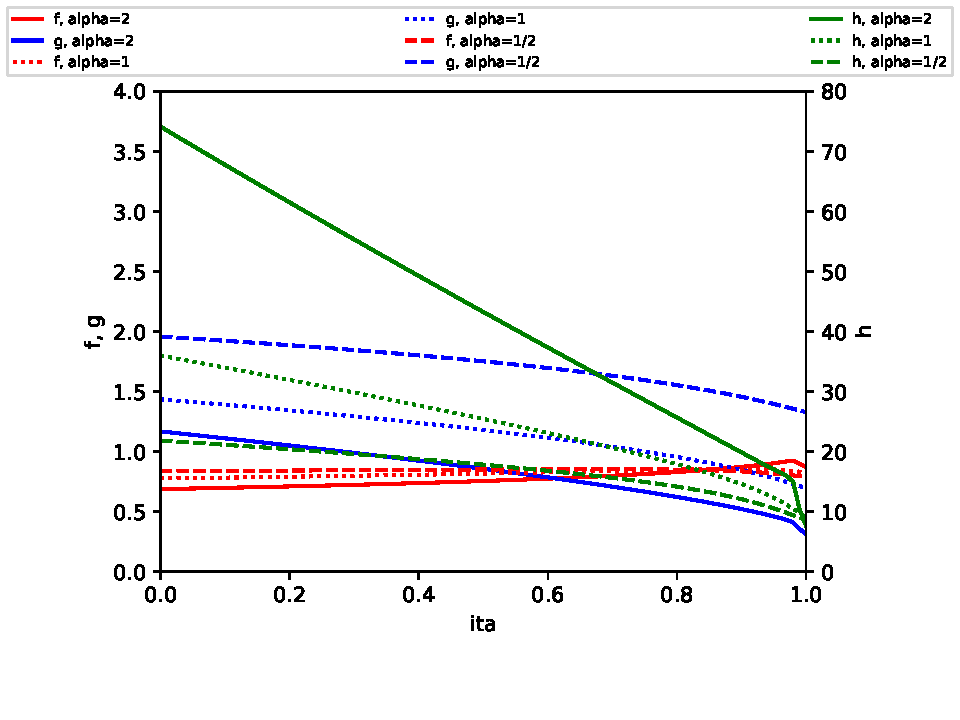
\includegraphics[scale=0.7]{gamma 1.2.png}}
\centerline{Figure 4.2: $\gamma$=$\frac{6}{5}$, Sakurai}

\newpage
\section*{4. Comments}
As shown in the plots above, the reproduced results generally match Sakurai's findings. The resulting values at $\eta=1$ also agree with the boundary conditions we obtained earlier with  relatively small errors. 
\bigbreak
Similar plots could be obtained for the second part of the problem, where the initial conditions are supposed to be found from the plots above when $\eta=0$.
\bigbreak
I was only able to partially finish this project, as further understanding of the theories used in Sakurai's work is much needed. On the other hand, I also need more coding practice in order to find the correct solutions in a more efficient manner. The current script I wrote need to be optimized in many ways, including finding a working method to solve the boundary value problem.
\bigbreak
This project would be a nice start for the rest of my summer research at CITA as the study of shock wave behaviors is a primary focus. 

\end{document}